\documentclass[aps,prd,twocolumn,superscriptaddress,nofootinbib,longbibliography,floatfix,amsmath,amssymb,showkeys,10pt]{revtex4-2}

\usepackage{mathptmx}
\usepackage{amsthm}
\usepackage{graphicx}
\usepackage{booktabs}
\usepackage{xcolor}
\usepackage{enumitem}
\usepackage[colorlinks=true,linkcolor=blue!50!black,citecolor=blue!50!black,urlcolor=blue!50!black,bookmarksnumbered=true]{hyperref}
\newcommand{\orcidlink}[1]{\href{https://orcid.org/#1}{\textcolor{green!45!black}{\textsuperscript{\sffamily iD}}}}
\usepackage{microtype}

\makeatletter
\AtBeginDocument{\def\NAT@bibsetup{\setlength{\labelwidth}{\z@}%
 \setlength{\labelsep}{0.5em}\setlength{\itemindent}{\z@}%
 \setlength{\listparindent}{\z@}\setlength{\topsep}{\z@}%
 \setlength{\parsep}{\z@}\NATx@bibsetup}}
\let\write@bibliographystyle\relax
\let\bibliography@latex\@gobble
% Widths of the section numbers and page numbers in the contents, so that
% the contents is set correctly from the second pass on.
\AtBeginDocument{%
 \@ifundefined{tocmax@section}{\gdef\tocmax@section{24.3pt}}{%
  \ifdim\tocmax@section<24.3pt\gdef\tocmax@section{24.3pt}\fi}%
 \@ifundefined{tocmax@pagenum}{\gdef\tocmax@pagenum{10pt}}{%
  \ifdim\tocmax@pagenum<10pt\gdef\tocmax@pagenum{10pt}\fi}}
\makeatother

\raggedbottom
\setlist{beginpenalty=0,midpenalty=0,endpenalty=0}
\makeatletter
\@beginparpenalty=0 \@endparpenalty=0 \@itempenalty=0
\setlength{\parskip}{0pt}
\makeatother
\tolerance=2000
\emergencystretch=3em
\hbadness=2000
\hfuzz=1pt

\newtheorem{theorem}{Theorem}
\newtheorem{lemma}[theorem]{Lemma}
\newtheorem{proposition}[theorem]{Proposition}
\newtheorem{corollary}[theorem]{Corollary}
\theoremstyle{definition}
\newtheorem{definition}[theorem]{Definition}
\newtheorem{conjecture}[theorem]{Conjecture}
\newtheorem{example}[theorem]{Example}
\theoremstyle{remark}
\newtheorem{remark}[theorem]{Remark}

\newcommand{\R}{\mathbb{R}}
\newcommand{\Z}{\mathbb{Z}}
\newcommand{\KS}{\mathrm{KS}}
\newcommand{\ip}[2]{\langle #1,#2\rangle}
\newcommand{\conv}{\operatorname{conv}}
\newcommand{\nvol}{\operatorname{nvol}}
\DeclareMathOperator{\Hom}{Hom}
\newcommand{\Tinf}{T^{\infty}}
\newcommand{\Dbig}{\Delta_{680}}
\newcommand{\UB}{348}
\newcommand{\UBplus}{349}
\newcommand{\LB}{22}
\newcommand{\DUB}{31}
\newcommand{\ZDOI}{}
\newcommand{\repolink}{\ifx\ZDOI\empty\url{https://github.com/creelie/seed}\else\href{https://doi.org/\ZDOI}{doi:\ZDOI}\fi}

\begin{document}

\title{Reflexive Descent to Minimal Seeds in the Kreuzer--Skarke List}

\author{Deep Bhattacharjee\,\orcidlink{0000-0003-0466-750X}}
\email{itsdeep@live.com}
\thanks{Corresponding author; second e-mail address
\nolinkurl{d.bhattacharjee@erl-forschung.de}}
\affiliation{Formerly, Electro-Gravitational Space Propulsion Laboratory
(EGSPL), Bhubaneswar, Odisha 751030, India}
\affiliation{Formerly, University of Calcutta, Senate House, 87/1 College
Street, Kolkata 700073, West Bengal, India}

\author{Ushashi Bhattacharya\,\orcidlink{0009-0002-2254-3914}}
\email{rai.bhattacharya.in@gmail.com}
\affiliation{Formerly, National Taiwan University, Taipei 106319, Taiwan}

\date{19 October 2026}

\begin{abstract}
\itshape
Kreuzer and Skarke built the list of reflexive polytopes by growing it
from small seed polytopes. We ask how far a polytope can be from its seeds
when it is shrunk through reflexive polytopes only, one at a time and
without skipping any. Such a descent always exists and always ends at a
seed. In four dimensions no descent takes more than 348 steps, which
proves the conjecture of a uniform transition depth, and in two and three
dimensions the exact maxima are five and eleven. In four dimensions two
polytopes with thirty-seven lattice points need exactly twenty-two steps, so
the maximum lies between twenty-two and 348.
\par\medskip\upshape\noindent
\textit{2020 Mathematics Subject Classification.} Primary 52B20, 14M25;
Secondary 14J32, 06A07, 52-08.
\end{abstract}

\keywords{reflexive polytopes; Kreuzer--Skarke list; Calabi--Yau threefolds; lattice polytopes}

\maketitle

\makeatletter
\renewcommand\l@subsection[2]{}
\renewcommand\l@subsubsection[2]{}
\makeatother
\tableofcontents

\section{Introduction}\label{sec:intro}

A lattice polytope is reflexive when it contains the origin in its
interior and every facet lies on a hyperplane $\ip{x}{y}=-1$ with $y$ a
lattice vector; equivalently, its polar dual is again a lattice polytope.
Batyrev showed that a reflexive polytope $\Delta$ of dimension four gives a
family of Calabi--Yau threefolds, the anticanonical hypersurfaces in the
toric variety of the fan over the faces of $\Delta^*$, and that the
exchange of $\Delta$ and $\Delta^*$ is mirror symmetry~\cite{Bat94}.
Kreuzer and Skarke classified these polytopes: there are $16$ in dimension
two, $4{,}319$ in dimension three~\cite{KS98} and $473{,}800{,}776$ in
dimension four~\cite{KS00}, up to unimodular equivalence. We write $\KS_d$
for the list in dimension $d$.

The classification rests on a finiteness principle. A lattice polytope with
the origin in its interior is called \emph{minimal} when removing any one
of its vertices and taking the convex hull of the others loses that
property, and every reflexive polytope contains a minimal one spanned by
some of its vertices~\cite{KS97,KS00}. In dimension four Kreuzer and
Skarke worked with a sharper notion: a reflexive polytope is
\emph{r-minimal} when it contains no reflexive polytope other than itself,
and every reflexive polytope contains an r-minimal one. Both notions
describe the seeds from which the whole list is grown, and the question
studied here is how far a polytope is from its seeds.

The seed universality preprint~\cite{Bha26a} proposed that the list is
generated from at most $64$ seed orbits with Hodge numbers constant on each
orbit. A later note~\cite{Bha26b} refuted that proposal, kept what is true
near it, and isolated the following statement as the part that remained
open.

\begin{conjecture}[Uniform transition depth~\cite{Bha26b}]\label{conj:depth}
There is an absolute constant $D$ such that every $\Delta\in\KS_4$ is
connected to some minimal seed by a chain of at most $D$ subpolytope steps
$\Delta_i\supset\Delta_{i+1}$ in which every intermediate hull is
reflexive after unimodular equivalence. The stratification data suggest a
value of $D$ of order a few tens.
\end{conjecture}

The note also asserted that descent through reflexive polytopes alone is
not always possible, and offered a vertex-deletion chain with
non-reflexive intermediate hulls as the substitute. We show that the
assertion is false, prove the conjecture with an explicit constant, and
determine the constant exactly in dimensions two and three.

To make the statement precise we use the order of the reflexive polytopes
by inclusion. A reflexive polytope $\Gamma\subsetneq\Delta$ is a
\emph{cover} of $\Delta$ when no reflexive polytope lies strictly between
them.\footnote{Here and below all polytopes live in the same lattice $M$
and have the origin as their only interior lattice point; a subpolytope of
$\Delta$ is a lattice polytope contained in $\Delta$. Reflexivity of a
subpolytope is always meant with respect to $M$ and the origin, which is
the reading of ``after unimodular equivalence'' in
Conjecture~\ref{conj:depth}: a unimodular map that carries $\Gamma$ into
$\Delta$ fixes the origin and the lattice.} A \emph{reflexive descent} of
$\Delta$ is a chain
\[
\Delta=\Delta_0\supsetneq\Delta_1\supsetneq\cdots\supsetneq\Delta_k
\]
in which each $\Delta_{i+1}$ is a cover of $\Delta_i$ and $\Delta_k$ is
r-minimal. Its length is $k$, and the \emph{transition depth}
$\delta(\Delta)$ is the least length of a reflexive descent of $\Delta$.
A descent never skips a reflexive polytope, so it is the strictest form of
the chains in Conjecture~\ref{conj:depth}; without the cover condition
every polytope reaches a seed in one step, as we explain in
Section~\ref{sec:literal}. We write $D_d$ for the largest transition depth
in $\KS_d$, and $|P|$ for the number of lattice points of a polytope $P$.

\begin{theorem}\label{thm:A}
Every reflexive polytope has a reflexive descent, every reflexive descent
ends at an r-minimal polytope, and every r-minimal polytope contains a
minimal polytope. Hence every $\Delta\in\KS_4$ is joined to a minimal seed
by a chain in which every intermediate hull is reflexive and no reflexive
polytope fits between two consecutive members.
\end{theorem}

\begin{theorem}\label{thm:B}
No reflexive descent in dimension four has more than $\UB$ steps. More
precisely, every reflexive descent of $\Delta\in\KS_4$ has length at most
$\min(|\Delta|-6,\,680-|\Delta^*|)$ and at most the pair bound
$L(|\Delta|,|\Delta^*|)$ of Section~\ref{sec:counting}. The first number
never exceeds $654$ and the second never exceeds $\UB$, and each maximum
is attained by a single polytope. Hence $D_4\le\UB$, and
Conjecture~\ref{conj:depth} holds with $D=\UBplus$.
\end{theorem}

\begin{theorem}\label{thm:C}
$D_2=5$ and $D_3=11$. In dimension two the maximum is attained only by the
triangle with ten lattice points; in dimension three it is attained by
exactly two polytopes, with $35$ and $31$ lattice points, both of which are
contained in no larger reflexive polytope.
\end{theorem}

\begin{theorem}\label{thm:D}
The polytopes $P_1$ and $P_2$ of Section~\ref{ssec:depth22}, with $37$
lattice points each, have transition depth exactly $\LB$, and $P_1$ is
unimodularly equivalent to the polytope reached after ten steps of a
reflexive descent of the simplex $\Dbig$ with $680$ lattice points, the
largest reflexive polytope in dimension four. The transition depth of
$\Dbig$ is at most $\DUB$. Hence $\LB\le D_4\le\UB$.
\end{theorem}

Theorem~\ref{thm:B} bounds every descent, not only the shortest one, so it
also bounds the longest chain of covers below any polytope. The existence
of some constant $D$ is the easy part of the conjecture: the list is finite
and Theorem~\ref{thm:A} gives each polytope a descent. The content of
Theorem~\ref{thm:B} is that the constant can be read off from two numbers
attached to each polytope, its lattice points and the lattice points of
its dual, without examining any polytope. The guess of ``a few tens'' in
the conjecture is neither confirmed nor refuted. The exact values $5$ and
$11$ in lower dimension, the depth $\LB$ of two polytopes with thirty-seven
points and the descent of length $\DUB$ from the largest polytope are
consistent with it, but we do not know where $D_4$ lies between $\LB$ and
$\UB$.

Theorem~\ref{thm:A} is a short argument in the inclusion order
(Section~\ref{sec:literal}). Theorem~\ref{thm:B} counts lattice points on
both sides of the duality: along a descent the polytope loses points and
its dual gains them, and both counts must stay among the pairs that occur
in the list (Section~\ref{sec:counting}). For the lower bounds we need all
covers of a given polytope. Section~\ref{sec:cuts} describes them as cuts
along dual lattice points; the volume bound of Balletti, Kasprzyk and
Nill~\cite{BKN22} leaves finitely many cuts to try, and a climbing lemma
certifies one cover without listing the others. In dimension two these
tools give $D_2=5$ by hand, and in dimensions three and four they give the
exact values and constructions of Sections~\ref{sec:low}
and~\ref{sec:four}. A lower bound for a depth is a statement about every
descent, and in dimension four we prove it with a certificate: a finite set
of polytopes with their complete lists of covers and a bound attached to
each, subject to a condition that can be checked one polytope at a time
(Lemma~\ref{lem:certificate}). The polytopes $P_1$ and $P_2$ are skew
bipyramids over a three-dimensional reflexive tetrahedron, and their
certificate contains $5{,}592$ polytopes. Section~\ref{sec:open} lists what
remains open.

\subsection*{History}

Reflexive polytopes entered algebraic geometry through Batyrev's
construction of mirror pairs of Calabi--Yau hypersurfaces~\cite{Bat94};
the lattice-point formulas for $h^{1,1}$ and $h^{2,1}$ in that paper made
the polytopes themselves the objects of study. Kreuzer and Skarke set out
to list them. Their first paper~\cite{KS97} introduced the minimal
polytopes, showed that a minimal polytope is either a simplex or a union of
lower-dimensional simplices sharing the origin as an interior point, and
attached a weight system to each simplex, so that the minimal polytopes in
a given dimension come from finitely many combined weight systems. The
three-dimensional list of $4{,}319$ polytopes followed in
1998~\cite{KS98}. In dimension four the combined weight systems number
$201{,}346$, too many to use directly, and Kreuzer and Skarke replaced
minimality by r-minimality: only $308$ combined weight systems give
r-maximal polytopes, that is, duals of r-minimal ones, and together with
$25$ sublattice versions and $7$ exceptional polytopes they give the $340$
r-maximal reflexive polytopes of dimension four~\cite{KS00}. Every
reflexive four-polytope is a subpolytope of one of these, and the complete
list of $473{,}800{,}776$ was obtained by enumerating subpolytopes with the
program PALP~\cite{KS04}. The lattice-point counts range from $6$ to
$680$~\cite{KS00}.

The inclusion order was used from the start to argue that the Calabi--Yau
hypersurfaces form a connected web. Candelas, Green and H\"ubsch had shown
that the complete intersections in products of projective spaces are
connected by conifold transitions~\cite{CGH90}; Avram, Kreuzer, Mandelberg
and Skarke showed that the toric hypersurfaces from weighted projective
spaces form a web connected by inclusions of polytopes~\cite{AKMS97}; and
Kreuzer and Skarke observed that connectedness of all reflexive
four-polytopes reduces to connectedness of the $340$ r-maximal ones, which
they checked during the classification~\cite{KS00}. Reid's question whether
all Calabi--Yau threefolds lie in one family connected by such
transitions~\cite{Rei87} remains open in general. Databases built on the
list~\cite{AGHJN15} made the joint statistics of polytopes and Hodge
numbers easy to read, and the list is now distributed in a form that can be
streamed in a few minutes~\cite{HF4D}.

The extremes of the list have a separate history. Lagarias and Ziegler
bounded the volume of lattice polytopes with a fixed number of interior
points~\cite{LZ91}; for reflexive polytopes the sharp bound was proved by
Balletti, Kasprzyk and Nill~\cite{BKN22}, who showed that in every
dimension $d\ge4$ the largest reflexive polytope is a simplex built from
Sylvester's sequence. In dimension four it is the simplex $\Dbig$ with
$680$ lattice points, the Newton polytope of the hypersurface of degree
$84$ in the weighted projective space $\mathbb{P}(1,1,12,28,42)$, whose
mirror is the Calabi--Yau threefold with the largest value of $h^{1,1}$ in
the list.

The question of distance to the seeds came from the seed universality
preprint~\cite{Bha26a}. Its orbit picture combined polar duality, stellar
subdivision and flips, and claimed constant Hodge numbers on at most $64$
orbits; the correcting note~\cite{Bha26b} disposed of that claim with two
observations (duality exchanges the Hodge pairs $(1,101)$ and $(101,1)$ of
the quintic and its mirror, and the list realises $30{,}108$ Hodge pairs),
proved the statements that survive at a fixed polytope, and stated
Conjecture~\ref{conj:depth}. The present paper answers it. Related work of
the first author on Calabi--Yau geometry and the landscape
includes~\cite{Bha26c}.

\section{Reflexive polytopes and their order}\label{sec:prelim}

Let $M\cong\Z^d$ be a lattice, $N=\Hom(M,\Z)$ its dual and
$\ip{\cdot}{\cdot}$ the pairing. For a polytope $P\subset M_\R$ with the
origin in its interior the polar dual is
$P^*=\{y\in N_\R:\ip{x}{y}\ge-1\text{ for all }x\in P\}$. A lattice polytope
$\Delta$ is reflexive when $\Delta^*$ is a lattice polytope; then
$\Delta^{**}=\Delta$, the facets of $\Delta$ are the sets
$\{\ip{x}{v}=-1\}\cap\Delta$ for the vertices $v$ of $\Delta^*$, and the
origin is the only interior lattice point. For a reflexive $\Delta$ let
$R(\Delta)$ be the set of reflexive subpolytopes of $\Delta$.

\begin{lemma}\label{lem:basic}
Let $\Gamma\subsetneq\Delta$ be lattice polytopes with the origin in their
interiors. Then
\begin{enumerate}[label=\textup{(\roman*)},leftmargin=*]
\item $|\Gamma|<|\Delta|$;
\item $\Delta^*\subsetneq\Gamma^*$, and if both are reflexive then
$|\Delta^*|<|\Gamma^*|$;
\item $R(\Delta)$ is finite, and every element of $R(\Delta)$ other than
$\Delta$ lies in a cover of $\Delta$.
\end{enumerate}
\end{lemma}

\begin{proof}
(i) If every vertex of $\Delta$ lay in $\Gamma$, the convex hull $\Delta$
would lie in $\Gamma$; so some vertex of $\Delta$, a lattice point, is
missing from $\Gamma$. (ii) Polarity reverses inclusion and is injective
on polytopes with the origin inside, and (i) applies to the lattice
polytopes $\Delta^*\subsetneq\Gamma^*$. (iii) A reflexive subpolytope is
the convex hull of a set of lattice points of $\Delta$, so there are at
most $2^{|\Delta|}$ of them. Given $\Gamma\in R(\Delta)$ with
$\Gamma\ne\Delta$, a maximal element of
$\{\Gamma'\in R(\Delta):\Gamma\subseteq\Gamma'\ne\Delta\}$ exists by
finiteness and is a cover of $\Delta$.
\end{proof}

A polytope is r-minimal exactly when it has no cover. By
Lemma~\ref{lem:basic}(iii) a reflexive polytope that is not r-minimal has
at least one cover, and we will need all of them.

\section{The literal conjecture and reflexive descent}\label{sec:literal}

\begin{proof}[Proof of Theorem~\ref{thm:A}]
Let $\Delta$ be reflexive. If $\Delta$ is r-minimal the descent of length
zero will do. Otherwise Lemma~\ref{lem:basic}(iii) gives a cover
$\Delta_1$, and we repeat with $\Delta_1$. By Lemma~\ref{lem:basic}(i) the
number of lattice points drops at each step, so the process stops, and it
stops exactly at an r-minimal polytope. Any reflexive descent ends at an
r-minimal polytope by definition.

Let $\Delta_k$ be r-minimal and let $V$ be its vertex set. Remove vertices
from $V$ one at a time, keeping the origin in the interior of the convex
hull of what is left, until no vertex can be removed. The hull $S$ of the
remaining set is a minimal polytope, its vertices are vertices of
$\Delta_k$, and $S\subseteq\Delta_k$. If $S\ne\Delta_k$ the step
$\Delta_k\supsetneq S$ leaves no room for a reflexive polytope between the
two, because $\Delta_k$ has no reflexive subpolytope other than itself.
Appending this step to a reflexive descent gives the chain of the
theorem.
\end{proof}

Three readings of Conjecture~\ref{conj:depth} are now settled at once. If
a ``subpolytope step'' may be any inclusion, the chain
$\Delta\supsetneq S$ of the second paragraph applied to $\Delta$ itself
has no intermediate hull at all, and $D=1$; this is the minimal-polytope
theorem of Kreuzer and Skarke~\cite{KS97} restated. If the seeds are the
r-minimal polytopes, which are the seeds of the four-dimensional
classification~\cite{KS00}, a reflexive descent ends at a seed. If the
seeds are minimal polytopes, at most one further step is needed. In every
reading the chain length is controlled by the transition depth, which is
the quantity bounded in Theorem~\ref{thm:B}.\footnote{In dimensions two and
three we checked which r-minimal polytopes are themselves minimal. The
three r-minimal polygons are minimal; in dimension three, twelve of the
sixteen r-minimal polytopes are minimal and four contain a smaller
minimal polytope that is not reflexive. In dimension four Kreuzer and
Skarke found seven r-minimal polytopes that do not come from weight
systems, and each of them contains a single minimal subpolytope, a simplex
that is not reflexive~\cite{KS00}.}

The correcting note~\cite{Bha26b} stated that descent through reflexive
polytopes only is not always possible. Theorem~\ref{thm:A} shows that it
always is. What fails is descent by deleting vertices, which is the
operation the note had in mind, and it fails in two ways.

\begin{proposition}\label{prop:vertexdeletion}
\begin{enumerate}[label=\textup{(\roman*)},leftmargin=*]
\item If $\Delta$ is a reflexive simplex, the convex hull of any proper
subset of its vertices is a face of $\Delta$ and contains no interior
point; so a reflexive simplex that is not r-minimal admits no descent by
convex hulls of vertex subsets, although it has a reflexive descent.
\item Among the $4{,}303$ reflexive three-polytopes that are not
r-minimal, exactly $74$ have no reflexive subpolytope of the form
$\conv\bigl((\Delta\cap M)\setminus\{v\}\bigr)$ with $v$ a vertex, and
exactly $354$ have none of the form $\conv(V\setminus\{v\})$ with $V$ the
vertex set.
\end{enumerate}
\end{proposition}

\begin{proof}
Part (i) is immediate: a proper subset of the vertices of a simplex spans
a face of positive codimension. Part (ii) is a finite check on the list of
Kreuzer and Skarke, recorded in the code archive~\cite{Repo}.
\end{proof}

\begin{example}\label{ex:vertexdeletion}
The smallest polytope in part (ii) has $15$ lattice points and vertices
$(1,0,0)$, $(0,1,0)$, $(-1,-1,0)$, $(0,0,1)$, $(-3,2,-2)$, $(-2,3,-2)$,
$(-4,4,-3)$. Removing any one vertex and taking the hull of the remaining
fourteen lattice points gives a polytope that is not reflexive, yet the
polytope has a reflexive descent of length $5$. In dimension four the
largest polytope $\Dbig$ is a simplex, so by part (i) it cannot be reduced
by vertex deletion at all, while Theorem~\ref{thm:D} gives it a descent of
length $36$.
\end{example}

The vertex-deletion chain of the note does reach a minimal polytope, and
its length is less than the number of vertices~\cite{Bha26b}; in dimension
four the vertex counts range from $5$ to $33$~\cite{KS00}, so such chains
have at most $28$ steps. Its intermediate hulls are not reflexive in
general, which is why the conjecture was stated with reflexive
intermediates.

\section{Counting lattice points}\label{sec:counting}

The lattice points of a polytope and of its dual move in opposite
directions along a descent, and in dimension four both counts are known for
every polytope of the list. This is enough to bound the length of every
descent. We write $\mathcal{P}_4\subset\Z^2$ for the set of pairs
$(|\Delta|,|\Delta^*|)$ with $\Delta\in\KS_4$; both numbers are invariant
under unimodular maps, and $\mathcal{P}_4$ is symmetric under
$(p,q)\mapsto(q,p)$ because the list is closed under duality.

\begin{definition}\label{def:pairbound}
For $(p,q)\in\mathcal{P}_4$ let $L(p,q)$ be the largest $k$ for which
there are pairs $(p_0,q_0),\dots,(p_k,q_k)$ in $\mathcal{P}_4$ with
$(p_0,q_0)=(p,q)$, $p_0>p_1>\cdots>p_k$ and $q_0<q_1<\cdots<q_k$. We call
$L(p,q)$ the \emph{pair bound} and write $L(\Delta)=L(|\Delta|,|\Delta^*|)$.
\end{definition}

The pair bound satisfies $L(p,q)=1+\max L(p',q')$ over the pairs with
$p'<p$ and $q'>q$, and $L(p,q)=0$ when there is no such pair. Evaluating
this recursion in increasing order of $p$ computes $L$ on all of
$\mathcal{P}_4$ at once.

\begin{lemma}\label{lem:counting}
Let $\Delta_0\supsetneq\Delta_1\supsetneq\cdots\supsetneq\Delta_k$ be
reflexive polytopes of dimension four, not necessarily a descent. Then
\[
k\;\le\;L(\Delta_0)\;\le\;\min\bigl(|\Delta_0|-6,\;680-|\Delta_0^*|\bigr).
\]
\end{lemma}

\begin{proof}
By Lemma~\ref{lem:basic} the counts $|\Delta_i|$ strictly decrease and the
counts $|\Delta_i^*|$ strictly increase. Each $\Delta_i$ is unimodularly
equivalent to a member of $\KS_4$, so each pair
$(|\Delta_i|,|\Delta_i^*|)$ lies in $\mathcal{P}_4$, and the pairs form a
chain as in Definition~\ref{def:pairbound}. Hence $k\le L(\Delta_0)$. In
any such chain of pairs the first coordinates are distinct integers between
$p_k$ and $p_0$ and the second are distinct integers between $q_0$ and
$q_k$. Every reflexive polytope of dimension four has at least six lattice
points and at most $680$~\cite{KS00}, which gives the second
inequality.\footnote{The lower bound six is elementary: a full-dimensional
lattice polytope in dimension four with an interior point has at least five
vertices, and the origin is a further lattice point. The upper bound $680$
is attained only by the simplex $\Dbig$ of Section~\ref{sec:four}, as the
list shows; Balletti, Kasprzyk and Nill proved that this simplex also has
the largest volume among reflexive four-polytopes~\cite{BKN22}.}
\end{proof}

The set $\mathcal{P}_4$ was computed by reading the two point counts of
all $473{,}800{,}776$ polytopes of the list~\cite{HF4D}. It has $71{,}870$
elements, its extreme values $6$ and $680$ agree with those recorded by
Kreuzer and Skarke~\cite{KS00}, and the counts add up to the size of the
list. Table~\ref{tab:counting} and Fig.~\ref{fig:pairs} summarise both
bounds over the list.

\begin{table*}[t]
\caption{Number of polytopes in $\KS_4$ whose bound on the length of a
reflexive descent exceeds a given value, for the simple bound
$\min(|\Delta|-6,680-|\Delta^*|)$ and for the pair bound $L(\Delta)$. The
last line gives the largest value of each bound and the point pair where it
is attained.}\label{tab:counting}
\begin{ruledtabular}
\begin{tabular}{lrrrrrrrrrr}
bound exceeds & $100$ & $150$ & $200$ & $250$ & $300$ & $320$ & $340$ & $348$ & $500$ & $654$\\
\hline
$\min(|\Delta|-6,680-|\Delta^*|)$ & $7{,}159{,}636$ & $893{,}324$ & $136{,}519$ & $30{,}306$ & $7{,}755$ & $4{,}763$ & $2{,}705$ & $2{,}197$ & $39$ & $0$\\
$L(\Delta)$ & $6{,}838{,}181$ & $825{,}559$ & $117{,}767$ & $23{,}814$ & $3{,}556$ & $1{,}028$ & $106$ & $0$ & $0$ & $0$\\
\hline
maximum & \multicolumn{10}{l}{simple bound $654$ at $(680,26)$, the simplex $\Dbig$; pair bound $348$ at $(521,22)$, a single polytope with seven vertices}\\
\end{tabular}
\end{ruledtabular}
\end{table*}

\begin{figure*}[t]
\centering
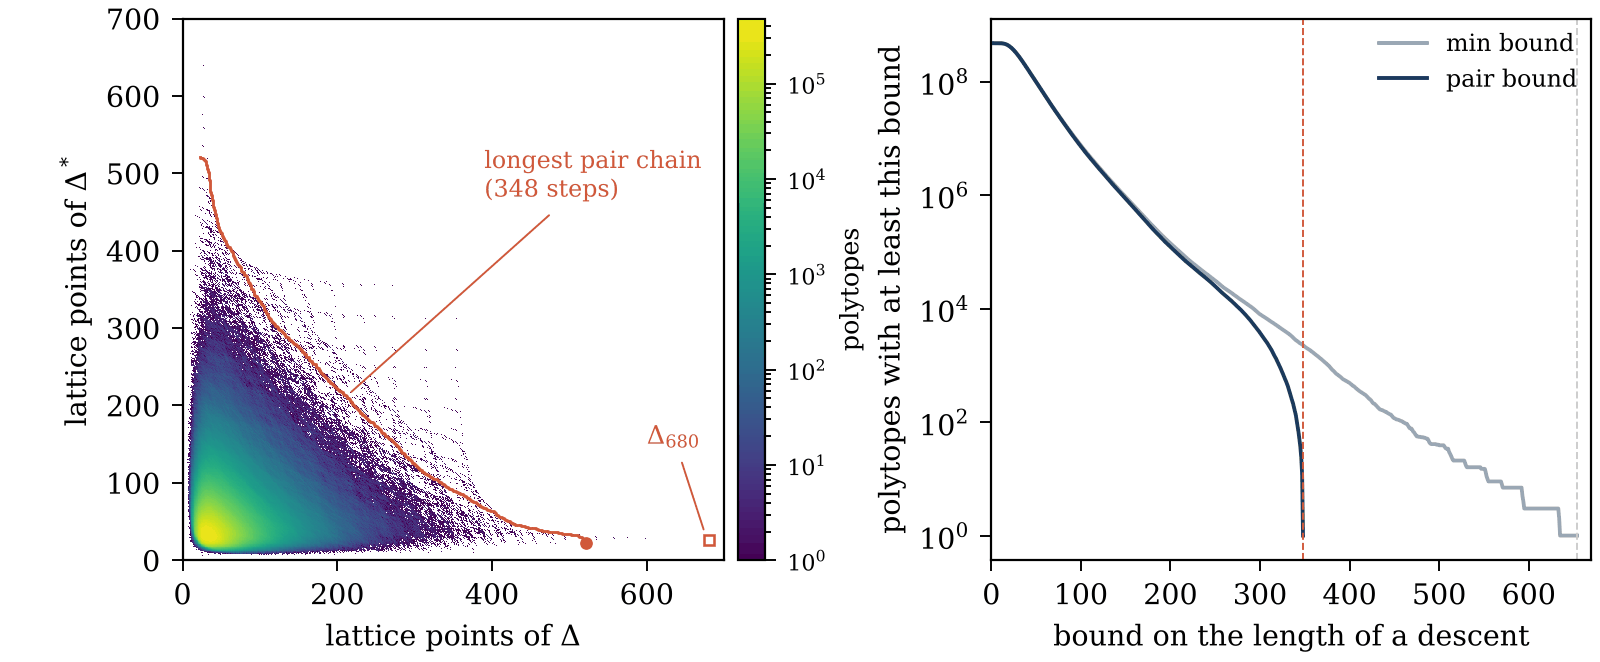
\includegraphics[width=\textwidth]{figures/fig_pairs.png}
\caption{Left: the number of reflexive four-polytopes with a given number
of lattice points (horizontal) and dual lattice points (vertical), on a
logarithmic colour scale. A reflexive descent moves left and up through
occupied cells. The red staircase is a longest chain of occupied cells,
with $348$ steps from $(521,22)$ to its mirror image $(22,521)$; the dot
marks its start and the square marks the simplex $\Dbig$ at $(680,26)$.
Right: for each value $X$, the number of polytopes whose bound on the
length of a descent is at least $X$, for the simple bound and the pair
bound.}\label{fig:pairs}
\end{figure*}

\begin{proof}[Proof of Theorem~\ref{thm:B}]
Lemma~\ref{lem:counting} applies to every reflexive descent. Over
$\mathcal{P}_4$ the largest value of $\min(p-6,680-q)$ is $654$, attained
only at $(680,26)$, and this pair belongs to one polytope, the simplex
$\Dbig$; the next values are $634$ at $(640,26)$ and $633$ at $(639,27)$.
The largest value of $L$ is $348$, attained only at $(521,22)$, again by a
single polytope, with vertices
\begin{multline*}
(1,0,0,0),\ (0,1,0,0),\ (0,0,1,0),\ (1,1,1,2),\\
(-3,-3,1,-2),\ (-45,-38,-6,-30),\ (15,22,-6,30)
\end{multline*}
and Hodge numbers $(h^{1,1},h^{2,1})=(10,376)$ for the hypersurface of
which it is the Newton polytope. So every reflexive descent in dimension
four has at most $\UB$ steps, $D_4\le\UB$, and with one more step to a
minimal polytope (Theorem~\ref{thm:A}) Conjecture~\ref{conj:depth} holds
with $D=\UBplus$.
\end{proof}

The pair bound of $\Dbig$ is $347$. A longest chain of pairs from
$(521,22)$ runs close to the upper edge of the occupied region and ends at
the mirror pair $(22,521)$ (Fig.~\ref{fig:pairs}). The chain is a property
of the point counts only; nothing in the argument says that a descent
follows it, and the descents we can compute are much shorter. For the
polytope at $(521,22)$, two covers found by the method of the next section
lead to a polytope with $257$ lattice points and $24$ dual points, whose
pair bound is $247$, so that polytope has a descent of length at most
$249$.

\section{Covers as cuts}\label{sec:cuts}

To compute transition depths we need all covers of a reflexive polytope.
In dimension two they are easy to list (Section~\ref{sec:low}), but in
dimension four a polytope can have hundreds of lattice points and
enumerating subsets is out of the question. The covers turn out to be cuts
by single dual lattice points, followed by a simple tightening operation.

For a lattice polytope $P$ with the origin in its interior put
\[
T(P)=\conv\{x\in P\cap M:\ \ip{x}{y}\ge-1\text{ for all }y\in P^*\cap N\}.
\]
If $T(P)$ again has the origin in its interior we may apply $T$ again; the
number of lattice points can only drop, so the sequence $P\supseteq
T(P)\supseteq T(T(P))\supseteq\cdots$ becomes constant, and we write
$\Tinf(P)$ for its final value. For a reflexive $\Delta$ and $q\in N$ put
\[
H_q=\conv\{x\in\Delta\cap M:\ \ip{x}{q}\ge-1\},
\]
the part of $\Delta$ that survives the cut by the hyperplane
$\ip{x}{q}=-1$.

\begin{lemma}[Cut lemma]\label{lem:cut}
Let $P$ be a lattice polytope with the origin in its interior and
$\Gamma\subseteq P$ a reflexive polytope. Then $\Gamma\subseteq T(P)$, so
$\Tinf(P)$ is defined and $\Gamma\subseteq\Tinf(P)$. If $P$ is reflexive,
then $T(P)=P$.
\end{lemma}

\begin{proof}
From $\Gamma\subseteq P$ we get $P^*\subseteq\Gamma^*$, so every
$y\in P^*\cap N$ lies in $\Gamma^*$ and satisfies $\ip{x}{y}\ge-1$ for all
$x\in\Gamma$. Hence every lattice point of $\Gamma$ is among the points
whose convex hull is $T(P)$, and $\Gamma$, being the convex hull of its
lattice points, lies in $T(P)$. In particular $T(P)$ has the origin in its
interior, and induction gives $\Gamma\subseteq\Tinf(P)$. If $P$ is
reflexive, every lattice point of $P$ satisfies $\ip{x}{y}\ge-1$ for every
$y\in P^*$, so nothing is removed.
\end{proof}

For a vertex $v$ of $\Delta$ let $F_v=\{y\in\Delta^*:\ip{v}{y}=-1\}$ be the
dual facet and $w_v=\nvol\conv(\{0\}\cup F_v)$ its normalised volume seen
from the origin, so that $\nvol\Delta^*=\sum_v w_v$. Let $V_d$ be the
largest normalised volume of a reflexive polytope of dimension $d$. The
classification gives $V_2=9$ and $V_3=72$, and Balletti, Kasprzyk and Nill
proved $V_4=2\cdot42^2=3528$, attained by $\Dbig$~\cite{BKN22}.

\begin{proposition}\label{prop:cuts}
Let $\Gamma$ be a cover of the reflexive polytope $\Delta\subset M_\R$ of
dimension $d$, and let $q$ be a vertex of $\Gamma^*$ that does not lie in
$\Delta^*$. Then
\begin{enumerate}[label=\textup{(\alph*)},leftmargin=*]
\item $q\in N$, and $\ip{v}{q}\le-2$ for some vertex $v$ of $\Delta$;
\item $\ip{x}{q}=-1$ for $d$ linearly independent lattice points $x$ of
$\Delta$;
\item $\sum_v w_v\max(1,-\ip{v}{q})\le V_d$, the sum running over the
vertices of $\Delta$;
\item $\Gamma\subseteq\Tinf(H_q)\subsetneq\Delta$, and either
$\Tinf(H_q)=\Gamma$, or $\Tinf(H_q)$ is not reflexive and $\Gamma$ is a
maximal reflexive polytope inside it.
\end{enumerate}
\end{proposition}

\begin{proof}
Since $\Gamma$ is reflexive, $\Gamma^*$ is a lattice polytope and its
vertex $q$ lies in $N$. As $q\notin\Delta^*=\{y:\ip{v}{y}\ge-1\text{ for
all vertices }v\}$, some vertex has $\ip{v}{q}<-1$, hence $\le-2$. This is
(a). The vertex $q$ of $\Gamma^*$ corresponds to a facet of $\Gamma$ lying
on the hyperplane $\ip{x}{q}=-1$. That facet is a lattice polytope of
dimension $d-1$, so it has $d$ affinely independent lattice points; they
are linearly independent because the hyperplane misses the origin, and
they are lattice points of $\Delta$. This is (b).

For (c), $\Gamma^*$ is a convex set containing $\Delta^*$ and $q$, so it
contains $C=\conv(\Delta^*\cup\{q\})$. The polytope $C$ is the union of
$\Delta^*$ and the pyramids with apex $q$ over the facets $F_v$ visible
from $q$, that is, those with $\ip{v}{q}<-1$, and these pieces meet only
along their boundaries. The lattice distance from $q$ to the hyperplane of
$F_v$ is $-\ip{v}{q}-1$, while the distance from the origin is $1$, so the
pyramid over $F_v$ has normalised volume $w_v(-\ip{v}{q}-1)$. Adding
$\nvol\Delta^*=\sum_v w_v$ gives $\nvol C=\sum_v w_v\max(1,-\ip{v}{q})$.
Since $\Gamma^*$ is reflexive, $\nvol C\le\nvol\Gamma^*\le V_d$.

For (d), every lattice point $x$ of $\Gamma$ lies in $\Delta$ and satisfies
$\ip{x}{q}\ge-1$ because $q\in\Gamma^*$; so $\Gamma\subseteq H_q$, and the
cut lemma gives $\Gamma\subseteq\Tinf(H_q)$. The vertex $v$ of (a) is a
lattice point of $\Delta$ that is not in $H_q$, so $\Tinf(H_q)\subseteq
H_q\subsetneq\Delta$. If $\Tinf(H_q)$ is reflexive, it lies strictly
between $\Gamma$ and $\Delta$ or equals $\Gamma$, and the first is excluded
because $\Gamma$ is a cover. Otherwise any reflexive $\Gamma'$ with
$\Gamma\subseteq\Gamma'\subseteq\Tinf(H_q)$ satisfies
$\Gamma\subseteq\Gamma'\subsetneq\Delta$, so $\Gamma'=\Gamma$.
\end{proof}

Conditions (a) and (c) confine $q$ to a bounded set: by (c) each
$-\ip{v}{q}$ is at most $V_d/w_v$, and the vertices of $\Delta$ span $M_\R$
positively. So only finitely many cuts have to be tried.

\begin{corollary}\label{cor:covers}
Let $\mathcal{C}(\Delta)$ be the set of reflexive polytopes obtained as
follows: for every $q$ satisfying (a), (b) and (c), take $\Tinf(H_q)$ if it
is reflexive, and otherwise its maximal reflexive subpolytopes. The covers
of $\Delta$ are exactly the maximal elements of $\mathcal{C}(\Delta)$
under inclusion.
\end{corollary}

\begin{proof}
Every element of $\mathcal{C}(\Delta)$ is a reflexive polytope strictly
inside $\Delta$, and by Proposition~\ref{prop:cuts} every cover belongs to
$\mathcal{C}(\Delta)$. A cover is maximal among all reflexive proper
subpolytopes, hence maximal in $\mathcal{C}(\Delta)$. Conversely, a maximal
element $X$ of $\mathcal{C}(\Delta)$ lies in some cover $C$ by
Lemma~\ref{lem:basic}(iii), and $C\in\mathcal{C}(\Delta)$, so $X=C$.
\end{proof}

Fig.~\ref{fig:cut} shows a cut in dimension two. In dimensions two and
three every polytope $\Tinf(H_q)$ that arose was reflexive, and so was
every one in the four-dimensional cases we checked. We do not know whether
the second case of Proposition~\ref{prop:cuts}(d) can occur at all; the
programs allow for it and then find the maximal reflexive subpolytopes by
removing vertices one at a time.

\begin{figure}[t]
\centering
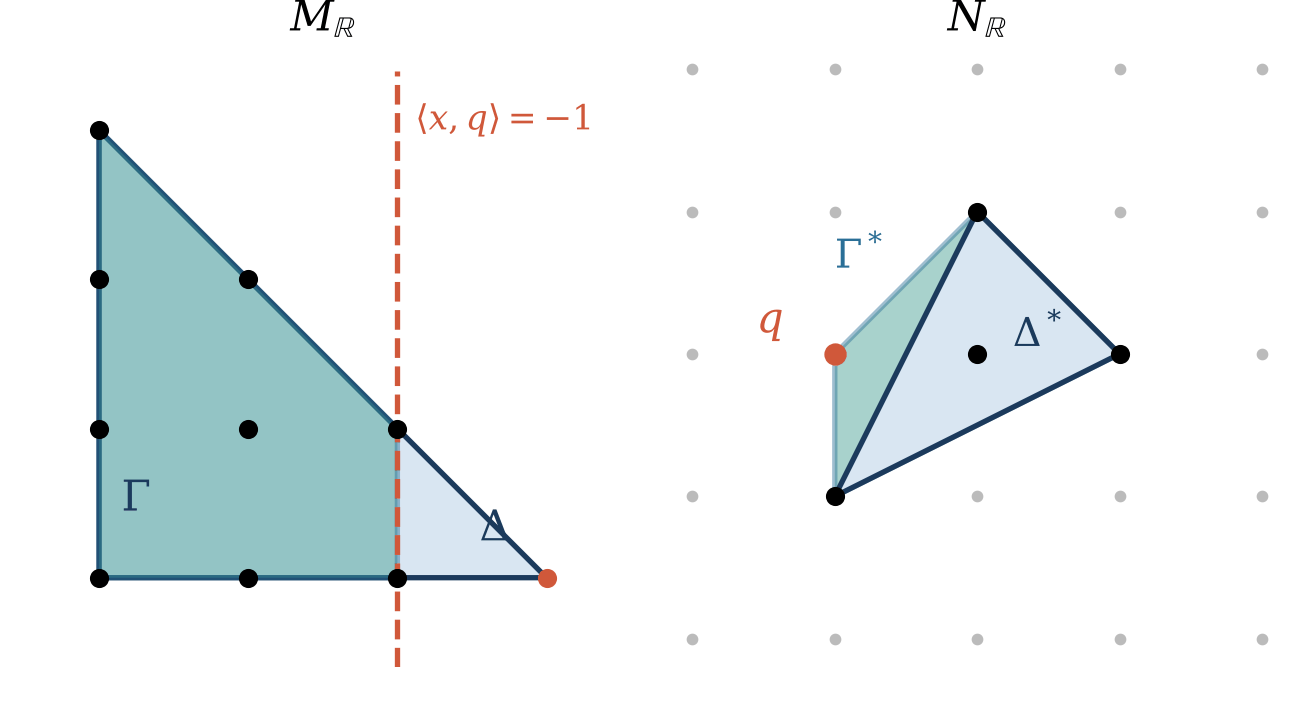
\includegraphics[width=\columnwidth]{figures/fig_cut.png}
\caption{A cover as a cut. Left: a reflexive triangle $\Delta$ with ten
lattice points and the cover $\Gamma$ (shaded) obtained by removing the
lattice points with $\ip{x}{q}<-1$. Right: the duals; $\Gamma^*$ is
$\Delta^*$ with the new vertex $q$, and the added piece is the pyramid of
Proposition~\ref{prop:cuts}(c) over the facet of $\Delta^*$ visible from
$q$.}\label{fig:cut}
\end{figure}

Listing all covers is still expensive for the largest polytopes. To walk
down from a polytope it is enough to certify one cover at a time, and for
that the following lemma needs only the dual lattice points of the
candidate.

\begin{lemma}[Climbing lemma]\label{lem:climb}
Let $\Gamma\subsetneq\Delta$ be reflexive. If $\Tinf(H_{q'})=\Gamma$ for
every lattice point $q'$ of $\Gamma^*$ outside $\Delta^*$, then $\Gamma$ is
a cover of $\Delta$.
\end{lemma}

\begin{proof}
Suppose $\Gamma\subsetneq\Gamma'\subsetneq\Delta$ with $\Gamma'$ reflexive.
Then $\Delta^*\subsetneq\Gamma'^*\subsetneq\Gamma^*$, so the lattice
polytope $\Gamma'^*$ has a vertex $q'\notin\Delta^*$, and $q'$ is a lattice
point of $\Gamma^*$. As in the proof of Proposition~\ref{prop:cuts}(d),
$\Gamma'\subseteq H_{q'}$ and the cut lemma gives
$\Gamma'\subseteq\Tinf(H_{q'})=\Gamma$, a contradiction.
\end{proof}

The lemma turns into a procedure. Start from a cut $q$ with $\Tinf(H_q)$
reflexive. For each lattice point $q'$ of $\Gamma^*$ outside $\Delta^*$,
the polytope $\Tinf(H_{q'})$ contains $\Gamma$ by the cut lemma; if it is
reflexive and larger, replace $\Gamma$ by it and start again. Since the
polytopes grow inside $\Delta$, this stops, and by the lemma the final
$\Gamma$ is a cover. Choosing the first cut so that $\Gamma$ is small
gives descents that lose many points per step, which is how the descent
of Section~\ref{sec:four} was found.

\section{Dimensions two and three}\label{sec:low}

In dimension two covers are simple.

\begin{proposition}\label{prop:twod}
If $\Gamma$ is a cover of a reflexive polygon $\Delta$, then
$|\Gamma|=|\Delta|-1$. Every r-minimal polygon $E\subseteq\Delta$ is the
last member of some reflexive descent of $\Delta$, and the transition depth
of a reflexive polygon is $\delta(\Delta)=|\Delta|-m(\Delta)$, where
$m(\Delta)$ is the largest number of lattice points of an r-minimal polygon
inside $\Delta$.
\end{proposition}

\begin{proof}
A lattice polygon with exactly one interior lattice point is
reflexive~\cite{PRV00}. Let $\Gamma\subsetneq\Delta$ be reflexive. Some
vertex $v$ of $\Delta$ is not in $\Gamma$, and
$\Delta'=\conv\bigl((\Delta\cap M)\setminus\{v\}\bigr)$ contains $\Gamma$,
hence the origin in its interior, and has no other interior lattice point;
so $\Delta'$ is reflexive, contains $\Gamma$, and has exactly
$|\Delta|-1$ lattice points, since a vertex is not in the hull of the
other lattice points. If $\Gamma$ is a cover, then $\Gamma=\Delta'$.

The same argument, applied to any reflexive $P$ with $E\subsetneq
P\subseteq\Delta$ and a vertex of $P$ outside $E$, gives a cover of $P$
that still contains $E$, so repeating it gives a descent of $\Delta$ that
ends at $E$, of length $|\Delta|-|E|$. Every descent loses one point per
step and ends at an r-minimal polygon, which gives the formula.
\end{proof}

\begin{proof}[Proof of Theorem~\ref{thm:C} in dimension two]
There are sixteen reflexive polygons, listed in Appendix~\ref{app:twod}
with their covers; three are r-minimal, the square
$\conv(\pm e_1,\pm e_2)$ and the triangle with vertices $(1,0)$, $(0,1)$,
$(-2,-1)$ with five lattice points each, and the triangle with vertices
$(1,0)$, $(0,1)$, $(-1,-1)$ with four. Every polygon with at least six
lattice points contains one of the two r-minimal polygons with five points
(the table names one), so by Proposition~\ref{prop:twod} its transition
depth is $|\Delta|-5$. The largest polygon is the triangle
$\conv\{(-1,-1),(2,-1),(-1,2)\}$ with ten lattice points; it contains the
square, so its depth is $5$, and every other polygon has at most nine
points and depth at most $4$. Hence $D_2=5$, attained only by this
triangle. It also contains the triangle with four points, so its longest
descent has $6$ steps.
\end{proof}

Fig.~\ref{fig:hasse2} shows the whole order. The argument uses only that
in the plane one interior point forces reflexivity; that fails from
dimension three on, and there covers can drop many points at once.

\begin{figure}[t]
\centering
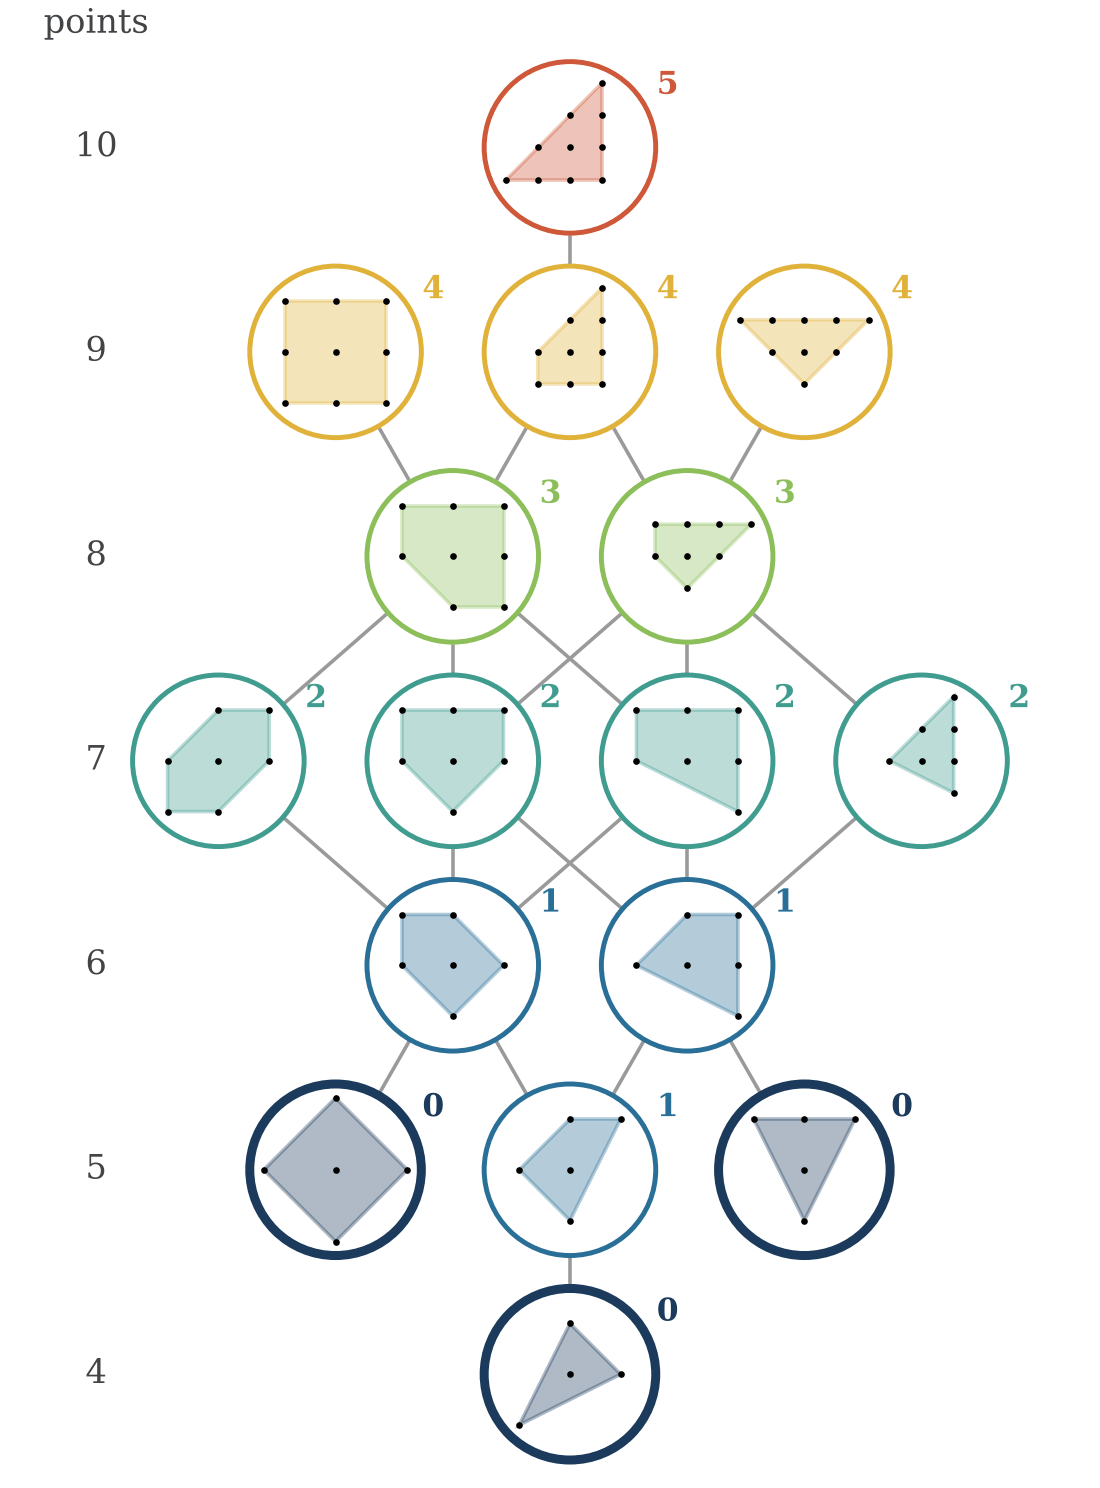
\includegraphics[width=0.86\columnwidth]{figures/fig_hasse2.png}
\caption{The sixteen reflexive polygons ordered by inclusion, by number of
lattice points; edges are covers and the number beside each polygon is its
transition depth. The three r-minimal polygons are drawn with thick
circles.}\label{fig:hasse2}
\end{figure}

In dimension three we computed the covers of all $4{,}319$ reflexive
polytopes in two independent ways. The first enumerates, for each
polytope, all lattice polytopes obtained by repeatedly removing a vertex
and taking the convex hull of the remaining lattice points, as long as the
origin stays inside; up to unimodular equivalence this gives $665{,}599$
polytopes, among them every reflexive subpolytope, and the covers are read
off as maximal elements. The second uses Corollary~\ref{cor:covers} with
$V_3=72$. The two agree on all $4{,}303$ polytopes that are not r-minimal,
and give $21{,}841$ covers in all.

\begin{proof}[Proof of Theorem~\ref{thm:C} in dimension three]
With the cover relation known, transition depths follow by induction on
the number of lattice points: $\delta(\Delta)=0$ if $\Delta$ has no cover
and $\delta(\Delta)=1+\min\delta(\Gamma)$ over its covers otherwise. The
maximum is $11$, attained by exactly two polytopes. The first has $35$
lattice points and vertices
\begin{gather*}
(1,0,0),\ (1,2,0),\ (-3,-2,0),\\
(1,2,4),\ (-3,-2,-4),
\end{gather*}
and the second has $31$ lattice points and vertices
\begin{gather*}
(1,0,0),\ (0,1,0),\ (1,0,2),\\
(1,-4,-2),\ (-2,3,2),\ (-2,-1,-2).
\end{gather*} Neither is contained in a larger
reflexive polytope, and both have longest descents of $23$ steps.
\end{proof}

The distribution of depths in dimension three is shown in
Fig.~\ref{fig:depth3}. The longest descent of any three-polytope has $28$
steps, against a simple counting bound of $33$, and sixteen polytopes are
r-minimal. Shortest and longest descents differ a great deal. The mean
transition depth is $5.67$, while the mean length of a longest descent is
$10.23$, so a well-chosen descent is on average a little more than half as
long as a badly chosen one.

\begin{figure*}[t]
\centering
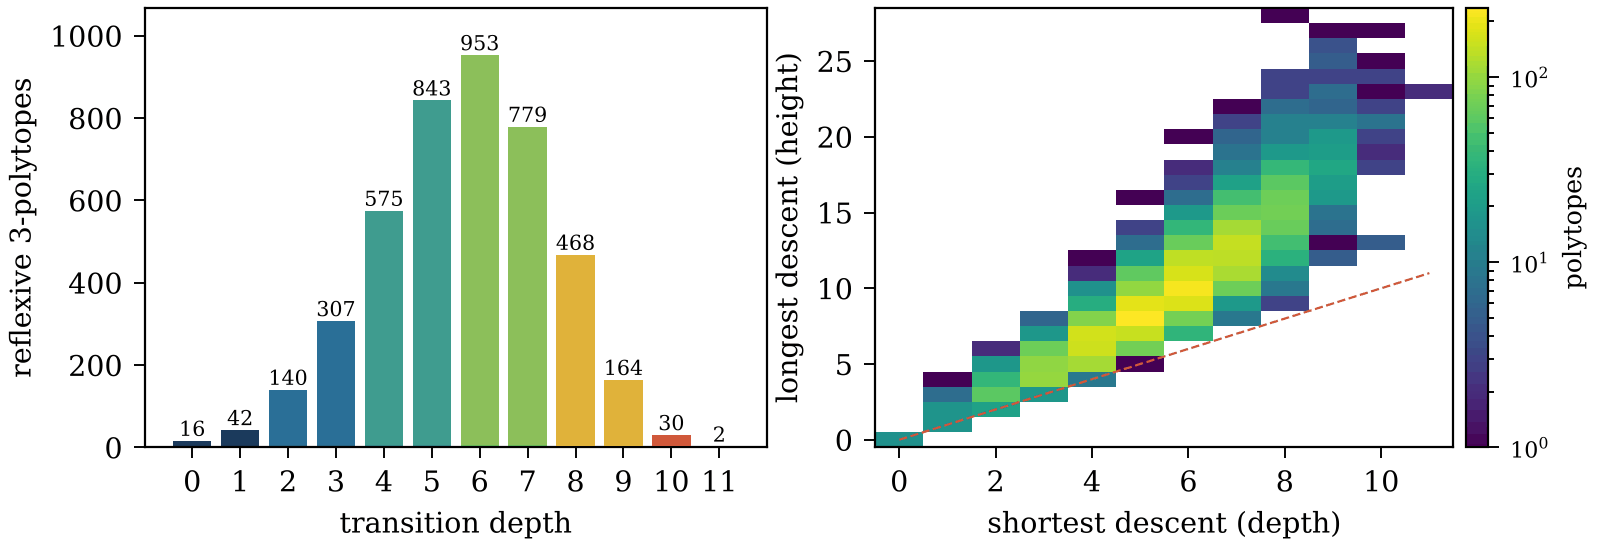
\includegraphics[width=\textwidth]{figures/fig_depth3.png}
\caption{Reflexive three-polytopes. Left: the number of polytopes with
each transition depth. Right: transition depth against the length of the
longest descent, with the diagonal dashed.}\label{fig:depth3}
\end{figure*}

\section{Dimension four}\label{sec:four}

\begin{table*}[t]
\caption{The sixteen reflexive polygons. Here $|\Delta|$ is the number of
lattice points, $c$ the number of covers, $\delta$ the transition depth and
$h$ the length of a longest descent; the last column gives an r-minimal
subpolygon with five lattice points. The three r-minimal polygons are the
last two rows with five points and the row with four.}\label{tab:twod}
\begin{ruledtabular}
\begin{tabular}{llrrrl}
vertices of $\Delta$ & $|\Delta|$ & $c$ & $\delta$ & $h$ & five-point r-minimal polygon inside $\Delta$\\
\hline
$(-2,-3)$, $(1,0)$, $(1,3)$ & $10$ & $1$ & $5$ & $6$ & $(-1,-2)$, $(0,1)$, $(1,0)$\\
$(-2,1)$, $(0,1)$, $(1,-2)$, $(1,0)$ & $9$ & $2$ & $4$ & $5$ & $(-2,1)$, $(0,1)$, $(1,-1)$\\
$(-1,-2)$, $(-1,0)$, $(1,0)$, $(1,2)$ & $9$ & $1$ & $4$ & $5$ & $(-1,-2)$, $(0,1)$, $(1,0)$\\
$(-3,-2)$, $(1,0)$, $(1,2)$ & $9$ & $1$ & $4$ & $5$ & $(-2,-1)$, $(0,1)$, $(1,0)$\\
$(-1,-2)$, $(-1,1)$, $(0,1)$, $(1,0)$ & $8$ & $3$ & $3$ & $4$ & $(-1,-2)$, $(0,1)$, $(1,0)$\\
$(-1,-1)$, $(-1,1)$, $(0,1)$, $(1,-1)$, $(1,0)$ & $8$ & $3$ & $3$ & $4$ & $(-1,-1)$, $(0,1)$, $(1,-1)$\\
$(-3,-2)$, $(0,1)$, $(1,0)$ & $7$ & $1$ & $2$ & $3$ & $(-2,-1)$, $(0,1)$, $(1,0)$\\
$(-1,-1)$, $(-1,1)$, $(0,-1)$, $(0,1)$, $(1,0)$ & $7$ & $2$ & $2$ & $3$ & $(-1,-1)$, $(-1,1)$, $(1,0)$\\
$(-2,1)$, $(0,-1)$, $(0,1)$, $(1,0)$ & $7$ & $2$ & $2$ & $3$ & $(-2,1)$, $(0,-1)$, $(1,0)$\\
$(-1,0)$, $(-1,1)$, $(0,-1)$, $(0,1)$, $(1,-1)$, $(1,0)$ & $7$ & $1$ & $2$ & $3$ & $(-1,1)$, $(0,-1)$, $(0,1)$, $(1,-1)$\\
$(-1,-1)$, $(-1,1)$, $(0,1)$, $(1,0)$ & $6$ & $2$ & $1$ & $2$ & $(-1,-1)$, $(-1,1)$, $(1,0)$\\
$(-1,0)$, $(0,-1)$, $(0,1)$, $(1,0)$, $(1,1)$ & $6$ & $2$ & $1$ & $2$ & $(-1,0)$, $(0,-1)$, $(0,1)$, $(1,0)$\\
$(-1,0)$, $(0,1)$, $(1,-1)$, $(1,0)$ & $5$ & $1$ & $1$ & $1$ & ---\\
$(-2,-1)$, $(0,1)$, $(1,0)$ & $5$ & $0$ & $0$ & $0$ & ---\\
$(-1,0)$, $(0,-1)$, $(0,1)$, $(1,0)$ & $5$ & $0$ & $0$ & $0$ & ---\\
$(-1,-1)$, $(0,1)$, $(1,0)$ & $4$ & $0$ & $0$ & $0$ & ---\\
\end{tabular}
\end{ruledtabular}
\end{table*}

\begin{table*}[t]
\caption{The reflexive descent $\Gamma_0=\Dbig\supsetneq\Gamma_1\supsetneq
\cdots\supsetneq\Gamma_{38}$: lattice points of $\Gamma_i$ and of
$\Gamma_i^*$, and vertices of $\Gamma_i$.}\label{tab:chain}
\begin{ruledtabular}
\begin{tabular}{rrrrcrrrrcrrrr}
$i$ & $|\Gamma_i|$ & $|\Gamma_i^*|$ & vert. & & $i$ & $|\Gamma_i|$ & $|\Gamma_i^*|$ & vert. & & $i$ & $|\Gamma_i|$ & $|\Gamma_i^*|$ & vert.\\
\hline
$0$ & $680$ & $26$ & $5$ & & $13$ & $34$ & $40$ & $6$ & & $26$ & $21$ & $88$ & $7$\\
$1$ & $422$ & $27$ & $7$ & & $14$ & $33$ & $42$ & $7$ & & $27$ & $20$ & $92$ & $7$\\
$2$ & $236$ & $28$ & $7$ & & $15$ & $32$ & $44$ & $7$ & & $28$ & $19$ & $104$ & $8$\\
$3$ & $207$ & $29$ & $9$ & & $16$ & $31$ & $46$ & $7$ & & $29$ & $18$ & $116$ & $8$\\
$4$ & $137$ & $30$ & $11$ & & $17$ & $30$ & $48$ & $7$ & & $30$ & $17$ & $128$ & $8$\\
$5$ & $122$ & $32$ & $9$ & & $18$ & $29$ & $51$ & $7$ & & $31$ & $16$ & $140$ & $8$\\
$6$ & $103$ & $33$ & $7$ & & $19$ & $28$ & $54$ & $7$ & & $32$ & $15$ & $152$ & $8$\\
$7$ & $78$ & $34$ & $9$ & & $20$ & $27$ & $58$ & $7$ & & $33$ & $14$ & $164$ & $7$\\
$8$ & $57$ & $35$ & $7$ & & $21$ & $26$ & $62$ & $7$ & & $34$ & $13$ & $179$ & $7$\\
$9$ & $44$ & $36$ & $7$ & & $22$ & $25$ & $66$ & $7$ & & $35$ & $12$ & $188$ & $7$\\
$10$ & $37$ & $37$ & $5$ & & $23$ & $24$ & $70$ & $7$ & & $36$ & $11$ & $196$ & $7$\\
$11$ & $36$ & $38$ & $6$ & & $24$ & $23$ & $80$ & $8$ & & $37$ & $10$ & $200$ & $6$\\
$12$ & $35$ & $39$ & $6$ & & $25$ & $22$ & $86$ & $8$ & & $38$ & $9$ & $201$ & $5$\\
\end{tabular}
\end{ruledtabular}
\end{table*}

The largest reflexive four-polytope is the simplex
\begin{multline*}
\Dbig=\conv\{(-1,-1,-1,-1),\,(83,-1,-1,-1),\\
(-1,6,-1,-1),\,(-1,-1,2,-1),\,(-1,-1,-1,1)\}.
\end{multline*}
Its lattice points are the exponents of the monomials of degree $84$ in
the weighted projective space $\mathbb{P}(1,1,12,28,42)$, shifted by the
interior point $(1,1,1,1)$, so it has $680$ lattice points. The dual
simplex has vertices $e_1,e_2,e_3,e_4$ and $(-1,-12,-28,-42)$, $26$
lattice points and normalised volume $1+1+12+28+42=84$, and $\Dbig$ has
normalised volume $3528=2\cdot42^2$, the largest possible~\cite{BKN22}.
The weights divided by their sum are $\tfrac12,\tfrac13,\tfrac17,
\tfrac1{84},\tfrac1{84}$, which add up to $1$ because
$\tfrac12+\tfrac13+\tfrac17+\tfrac1{42}=1$; here $2,3,7,43$ are the first
terms of Sylvester's sequence and $42=43-1$. The hypersurfaces have Hodge numbers
$(h^{1,1},h^{2,1})=(11,491)$, and their mirror has the largest $h^{1,1}$ in
the list.

Because $\Dbig$ is a simplex, no proper subset of its vertices spans a
polytope with the origin inside, so vertex deletion cannot even start
(Proposition~\ref{prop:vertexdeletion}). Reflexive descent works
(Fig.~\ref{fig:chain680}). Ten steps of the climbing procedure of
Section~\ref{sec:cuts} take the number of lattice points through
\[
680,\ 422,\ 236,\ 207,\ 137,\ 122,\ 103,\ 78,\ 57,\ 44,\ 37,
\]
each step certified as a cover by Lemma~\ref{lem:climb}. From $37$ points
on, all covers were computed by Corollary~\ref{cor:covers}; each step
removes one point, and after $38$ steps the descent reaches a simplex with
nine lattice points and vertices
\begin{gather*}
(-1,-1,-1,1),\ (-1,-1,2,-1),\ (-1,0,1,-1),\\
(-1,6,-1,-1),\ (1,0,0,0),
\end{gather*}
which has no reflexive subpolytope and is itself minimal. The dual counts
rise from $26$ to $201$ along the way. Appendix~\ref{app:chain} lists the
whole descent.

\begin{figure}[t]
\centering
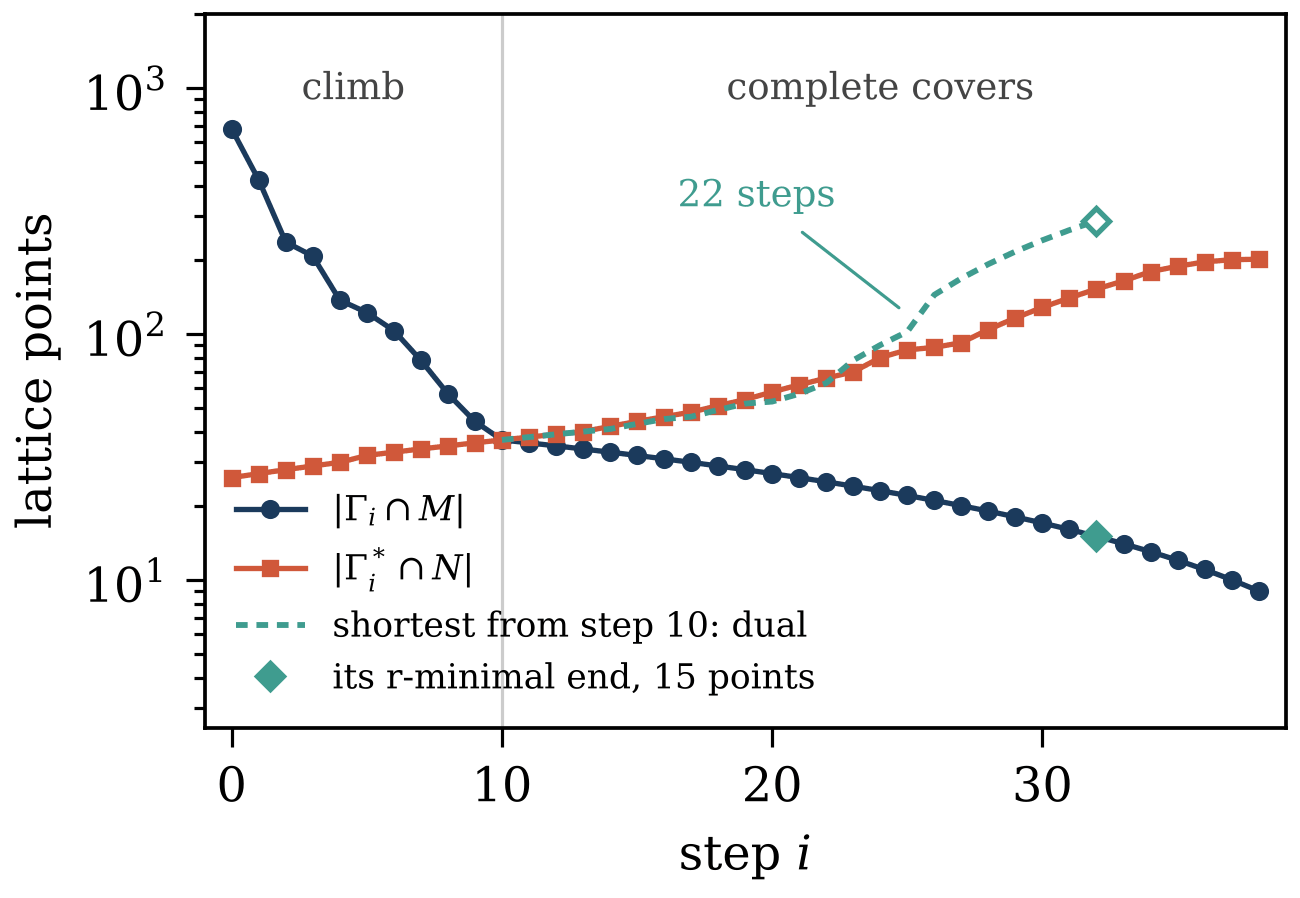
\includegraphics[width=\columnwidth]{figures/fig_chain680.png}
\caption{The descent from $\Dbig$: lattice points of $\Gamma_i$ and of its
dual at each step. The first ten covers were certified by the climbing
lemma, the remaining ones by listing all covers. The polytope $\Gamma_{10}$
is the polytope $P_1$ of Section~\ref{ssec:depth22}; a shortest descent of
it has $22$ steps, removes one lattice point at each step like the descent
drawn, and ends at an r-minimal polytope with $15$ lattice points (filled
diamond) whose dual has $288$ (open diamond). The dashed line shows its
dual counts.}
\label{fig:chain680}
\end{figure}

\subsection{A certificate for lower bounds}\label{ssec:certificate}

An upper bound for a transition depth needs one descent, a lower bound a
statement about all of them. The following lemma reduces a lower bound to
a finite object that can be checked one polytope at a time.

\begin{lemma}[Certificate lemma]\label{lem:certificate}
Let $\mathcal{N}$ be a set of reflexive polytopes and
$b\colon\mathcal{N}\to\mathbb{Z}_{\ge0}$ a function such that for every
$\Gamma\in\mathcal{N}$ with $b(\Gamma)>0$ the polytope $\Gamma$ has a
cover, and every cover of $\Gamma$ is unimodularly equivalent to some
$\Gamma'\in\mathcal{N}$ with $b(\Gamma')\ge b(\Gamma)-1$. Then
$\delta(\Gamma)\ge b(\Gamma)$ for every $\Gamma\in\mathcal{N}$.
\end{lemma}

\begin{proof}
A unimodular map fixes the lattice and the origin and preserves inclusion,
so it carries covers to covers and r-minimal polytopes to r-minimal ones;
hence $\delta$ is constant on classes of unimodularly equivalent
polytopes. We use induction on $|\Gamma|$. If $b(\Gamma)=0$ there is
nothing to prove. Otherwise $\Gamma$ has a cover, so it contains a
reflexive polytope other than itself and is not r-minimal, and every
descent $\Gamma=\Gamma_0\supsetneq\Gamma_1\supsetneq\cdots\supsetneq
\Gamma_k$ has $k\ge1$. Its first step $\Gamma_1$ is a cover of $\Gamma$,
so it is equivalent to some $\Gamma'\in\mathcal{N}$ with $b(\Gamma')\ge
b(\Gamma)-1$, and $|\Gamma'|=|\Gamma_1|<|\Gamma|$ by
Lemma~\ref{lem:basic}(i). The chain $\Gamma_1\supsetneq\cdots\supsetneq
\Gamma_k$ is a descent of $\Gamma_1$, so the induction hypothesis gives
$k-1\ge\delta(\Gamma_1)=\delta(\Gamma')\ge b(\Gamma')\ge b(\Gamma)-1$, and
$k\ge b(\Gamma)$.
\end{proof}

The lemma asks for a complete list of covers only at the polytopes with
positive bound, and Corollary~\ref{cor:covers} provides such lists. The
polytopes need not be the same as those of any particular descent, and the
bounds need not be exact depths. A certificate is produced by a bounded
search: to show $\delta(\Gamma)>\ell$ it lists the covers of $\Gamma$ and
shows $\delta(\Gamma')>\ell-1$ for each of them, identifying unimodularly
equivalent polytopes by their normal forms and keeping every bound it has
proved, so that a polytope reached along many paths is examined
once.\footnote{The search is a depth-first search with a memory of exact
depths and of lower bounds. For a bound $\ell$ it tries the covers of
$\Gamma$ in the order of their known depths, smallest first, and stops as
soon as one of them has depth at most $\ell-1$; if none has, the bound
$\delta(\Gamma)\ge\ell+1$ is recorded. Repeating with $\ell=0,1,2,\dots$
gives the exact depth, and the recorded bounds of all polytopes that were
reached form a function $b$ as in Lemma~\ref{lem:certificate}. Exact depths
found on the way are recorded as well; they give the descents that prove the
matching upper bounds.} The certificate is then checked by a program that
does not repeat the search: it verifies the hypothesis of the lemma
polytope by polytope and recomputes the lists of covers.

\subsection{Two polytopes of depth twenty-two}\label{ssec:depth22}

Let $e_1,\dots,e_4$ be the standard basis of $M=\mathbb{Z}^4$, put
$u=(-4,-2,-1,0)$, and let
\begin{align*}
P_1&=\conv\{e_1,\,e_2,\,e_3,\,u+8e_4,\,u-8e_4\},\\
P_2&=\conv\{e_1,\,e_2,\,e_3,\,u,\,u+8e_4,\,e_3-8e_4\}.
\end{align*}
Both polytopes contain $Q\times\{0\}$, where the tetrahedron
$Q=\conv\{e_1,e_2,e_3,(-4,-2,-1)\}$ lies in $\mathbb{R}^3$ with the
lattice $\mathbb{Z}^3$, and both are bipyramids over it with apexes
at height $\pm8$: $P_1$ is the convex hull of $Q\times\{0\}$ and the two
points $((-4,-2,-1),\pm8)$, and $P_2$ that of $Q\times\{0\}$ and the points
$((-4,-2,-1),8)$ and $(e_3,-8)$. The tetrahedron $Q$ is reflexive, it is the
simplex of the weights $(4,2,1,1)$ because $4e_1+2e_2+e_3+(-4,-2,-1)=0$, and
it has the seven lattice points
\[
e_1,\ e_2,\ e_3,\ (-4,-2,-1),\ (-2,-1,0),\ (-1,0,0),\ 0.
\]
It contains no reflexive polytope other than itself, so it is r-minimal
and its transition depth in dimension three is $0$.

The polytope $P_1$ is a simplex, and
$8e_1+4e_2+2e_3+(u+8e_4)+(u-8e_4)=0$, so it is the simplex of the weights
$(8,4,2,1,1)$. Its lattice points lie on vertical lines over the lattice
points of $Q$. A point $(x,t)$ with $x\in Q$ lies in $P_1$ exactly when
$|t|\le8\lambda(x)$, where $\lambda(x)$ is the barycentric coordinate of
$x$ in $Q$ at the vertex $(-4,-2,-1)$; indeed, writing
$(x,t)=\mu_1e_1+\mu_2e_2+\mu_3e_3+\alpha(u+8e_4)+\beta(u-8e_4)$ with
nonnegative coefficients of sum $1$ gives $\alpha+\beta=\lambda(x)$ and
$t=8(\alpha-\beta)$. The barycentric coordinates of the four lattice
points $(-4,-2,-1)$, $(-2,-1,0)=\tfrac12(-4,-2,-1)+\tfrac12e_3$,
$(-1,0,0)=\tfrac14(-4,-2,-1)+\tfrac12e_2+\tfrac14e_3$ and
$0=\tfrac18(-4,-2,-1)+\tfrac12e_1+\tfrac14e_2+\tfrac18e_3$ at that vertex
are $1,\tfrac12,\tfrac14,\tfrac18$, so the lines over them carry $17$,
$9$, $5$ and $3$ lattice points, and the three points $e_1,e_2,e_3$ carry
one each (Fig.~\ref{fig:depth22}(a)). Hence
\[
|P_1|=17+9+5+3+3=37.
\]
The dual simplex $P_1^*$ has the vertices $(-1,-1,-1,\pm1)$,
$(-1,-1,7,0)$, $(-1,3,-1,0)$ and $(1,-1,-1,0)$, read off from the five
facets of $P_1$, and it also has $37$ lattice points. The polytope $P_2$ has
six vertices, and $|P_2|=|P_2^*|=37$. For both polytopes the Calabi--Yau
hypersurfaces have Hodge numbers $(h^{1,1},h^{2,1})=(34,34)$.

\begin{figure*}[t]
\centering
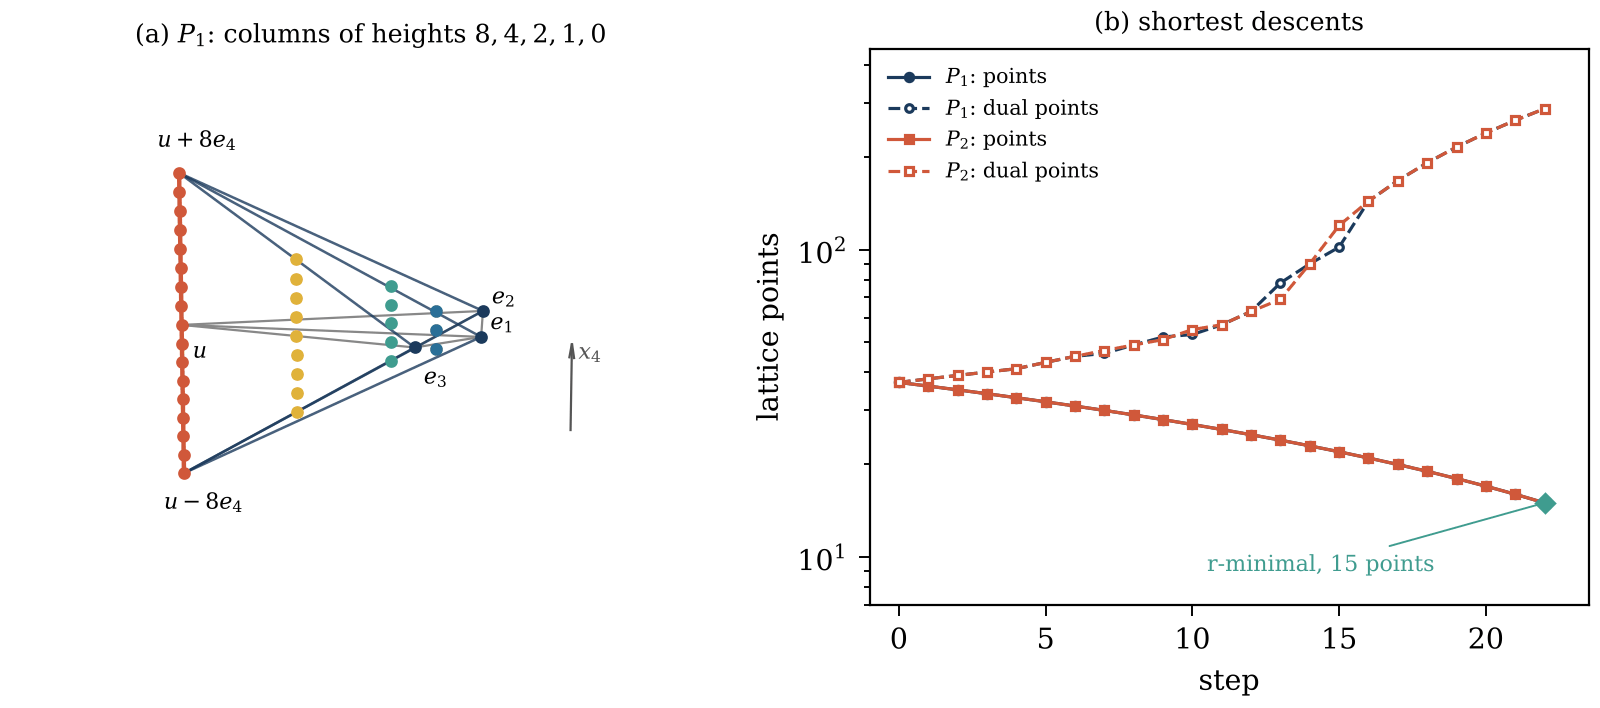
\includegraphics[width=\textwidth]{figures/fig_depth22.png}
\caption{(a) The polytope $P_1$ as a bipyramid over the tetrahedron
$Q\times\{0\}$ (grey edges), with the fourth coordinate vertical. Its $37$
lattice points lie on vertical lines over the seven lattice points of $Q$,
with $17$, $9$, $5$ and $3$ points over $(-4,-2,-1)$, $(-2,-1,0)$,
$(-1,0,0)$ and $0$ and one point at each of $e_1,e_2,e_3$; the half-lengths
$8,4,2,1,0$ of these lines are $8$ times the barycentric coordinate at the
vertex $(-4,-2,-1)$ of $Q$. (b) Lattice points (solid) and dual lattice
points (dashed) along shortest descents of $P_1$ and $P_2$. Each step
removes one lattice point, and both descents end at the same r-minimal
polytope, with $15$ lattice points and $288$ dual lattice points
(diamond).}\label{fig:depth22}
\end{figure*}

The two polytopes were found by a search over skew bipyramids
$\conv(Q'\times\{0\}\cup\{(a,k),(b,-k)\})$ over three-dimensional
reflexive polytopes $Q'$, with $a,b$ lattice points of $Q'$ and $k\ge1$,
ranked by the length of a descent found greedily with the cuts of
Section~\ref{sec:cuts}; the exact depths of the highest ranked were then
computed with complete lists of covers.\footnote{The search was organised
on the Anaxia engine of the BLLM programme~\cite{Ana26,BB26}, release
3.0.5. Anaxia runs a failure-driven loop: each strategy for a target is a
list of checks, a computation or a proof with a named source, a failed
check is recorded together with the change of strategy it forces, all
checks are rerun from the archived data, and the label of a target (open,
candidate, proved) is computed from the record, never assigned by hand.
For the upper bound of Theorem~\ref{thm:B} its record shows the first two
strategies failing: descent by deleting one vertex at a time fails on $7$
of $400$ sampled three-dimensional polytopes, which have no reflexive
vertex deletion, and cuts at dual lattice points of gauge two miss covers
on $73$ of the $400$; the change forced by the second failure was the
complete set of cuts of Corollary~\ref{cor:covers}, which agrees with the
vertex-deletion order on all of them. For the sharp form of
Conjecture~\ref{conj:depth} the first strategy, a sweep of the whole list,
failed on cost, since $162{,}328{,}050$ polytopes have
$\min(|\Delta|-6,680-|\Delta^*|)>40$; the second and third gave the descent
of $\Dbig$ with exact depths of small polytopes along it; the fourth was
the search over skew bipyramids that produced $P_1$ and $P_2$, with the
certificate of Proposition~\ref{prop:depth22} and the identification of
Proposition~\ref{prop:gamma10} as its checks. Its check that the sharp
constant is determined fails, and that target stays open. The engine
organises and reruns the computations; every statement of this section is
proved in the text, and the certificate is checked by the programs of
Appendix~\ref{app:checks}, which do not use the engine.}

\begin{proposition}\label{prop:depth22}
$\delta(P_1)=\delta(P_2)=22$.
\end{proposition}

\begin{proof}
For the upper bound, each of $P_1$ and $P_2$ has a descent of $22$ steps,
each step a cover by Corollary~\ref{cor:covers}. Both remove one lattice
point at each step, so the numbers of lattice points run through
$37,36,\dots,15$, while the dual counts rise from $37$ to $288$
(Fig.~\ref{fig:depth22}(b)). Both end at the same polytope, with vertices
\[
(-4,-2,-1,7),\ (-2,-1,0,-1),\ (-2,-1,0,4),\ e_1,\ e_2,\ e_3,
\]
$15$ lattice points and no cover.

For the lower bound we apply Lemma~\ref{lem:certificate} to a set
$\mathcal{N}$ of $5{,}592$ polytopes containing $P_1$ and $P_2$, with
$b(P_1)=b(P_2)=22$. Of these, $5{,}251$ have positive bound; for each of
them the set $\mathcal{N}$ contains a representative of every cover, given
by the complete list of Corollary~\ref{cor:covers}, $23{,}646$ covers in
all, and each cover has bound at least one less. The lemma gives
$\delta(P_1),\delta(P_2)\ge22$.
\end{proof}

The polytopes of the certificate have between $14$ and $37$ lattice
points; the most frequent sizes are $17$ to $20$ points, with between
$472$ and $494$ polytopes each, and only $61$ polytopes have more than
$31$ points.

\begin{proposition}\label{prop:gamma10}
The matrix
\[
G=\begin{pmatrix}-1&-1&-1&-1\\-1&-1&6&0\\-1&2&-1&0\\1&-1&-1&0\end{pmatrix}
\]
is unimodular, and $x\mapsto Gx$ carries $P_1$ onto the polytope
$\Gamma_{10}$ of the descent of $\Dbig$ in Table~\ref{tab:chain}. Hence
$\delta(\Gamma_{10})=22$ and $\delta(\Dbig)\le32$.
\end{proposition}

\begin{proof}
The matrix
\[
H=\begin{pmatrix}0&3&7&11\\0&2&5&7\\0&1&2&3\\-1&-6&-14&-21\end{pmatrix}
\]
is integral and $GH=1$, so $G$ is unimodular. The map sends $e_1$, $e_2$,
$e_3$, $u+8e_4$ and $u-8e_4$ to
\begin{gather*}
(-1,-1,-1,1),\ (-1,-1,2,-1),\ (-1,6,-1,-1),\\
(-1,0,1,-1),\ (15,0,1,-1),
\end{gather*}
which are the five vertices of the simplex $\Gamma_{10}$. Since
$\Gamma_{10}$ is reached from $\Dbig$ by ten covers,
$\delta(\Dbig)\le10+\delta(\Gamma_{10})=10+22$.
\end{proof}

Three of the vertices of $\Gamma_{10}$ are vertices of $\Dbig$, and the
other two lie on its facet $x_4=-1$. One step higher the same search gives
a descent of $22$ steps from $\Gamma_9$, which has $44$ lattice points: it
removes one or two points at a time and ends at an r-minimal polytope with
$19$ lattice points. Hence $\delta(\Dbig)\le9+22=\DUB$.

\begin{proof}[Proof of Theorem~\ref{thm:D}]
Proposition~\ref{prop:depth22} gives $\delta(P_1)=\delta(P_2)=\LB$, so
$D_4\ge\LB$, and Proposition~\ref{prop:gamma10} identifies $P_1$ with
$\Gamma_{10}$. The nine covers from $\Dbig$ to $\Gamma_9$ in
Table~\ref{tab:chain}, each certified by the climbing lemma,
followed by the descent of $22$ steps from $\Gamma_9$, form a descent of
$\Dbig$ of length $\DUB$. Finally $D_4\le\UB$ by Theorem~\ref{thm:B}.
\end{proof}

Smaller polytopes along the descent of $\Dbig$ have smaller depth: the
same search gives $\delta(\Gamma_{27})=9$ for the polytope with twenty
lattice points and $\delta(\Gamma_{32})=4$ for the one with fifteen, and
among the four-polytopes with at most eleven lattice points the largest
transition depth is $5$.

\section{Open questions}\label{sec:open}

The main open problem is the exact value of $D_4$. We know
$\LB\le D_4\le\UB$. The upper bound comes from point counts alone and is
attained by no descent that we know; the lower bound comes from two
polytopes with thirty-seven points, one of which lies ten covers below
$\Dbig$. Two improvements look within reach. The upper bound can be
lowered polytope by polytope: a few certified covers bring a polytope to
one with a small pair bound, as for the polytope at $(521,22)$ in
Section~\ref{sec:counting}, and only $106$ polytopes have pair bound above
$340$. The lower bound rises as soon as one polytope is found all of whose
covers have depth at least $\LB$, and Lemma~\ref{lem:certificate} turns
such a search into a checkable certificate. The reflexive polytopes that
contain $P_1$ or $P_2$, and the polytopes $\Gamma_9,\dots,\Gamma_1$ of the
descent of $\Dbig$, are the first candidates; the cost of the search lies
in listing covers of polytopes with many lattice points.

Three further questions seem natural. First, how does $D_d$ grow with the
dimension? The counting argument of Section~\ref{sec:counting} bounds $D_d$
in every dimension as soon as the joint distribution of point counts is
known, and that distribution is not known in dimension five.

Second, how far apart can the shortest and the longest descent of one
polytope be? In dimension two they differ by at most one. In dimension
three the largest difference is $20$, for the polytope with $35$ lattice
points, whose depth is $8$ and whose longest descent has $28$ steps
(Fig.~\ref{fig:depth3}).

Third, do the polytopes of maximal depth share a structure? In dimension
two the extreme polygon is the triangle of the weights $(1,1,1)$, and in
dimension three both extremes are r-maximal. In dimension four the
polytope $P_1$ is the simplex of the weights $(8,4,2,1,1)$ and lies inside
$\Dbig$, so it is not r-maximal; whether the polytope of largest depth in
dimension four is r-maximal is open.

\section*{Data availability}

The code and data behind every computation in this paper are in the
repository \url{https://github.com/creelie/seed}, whose releases are
archived at Zenodo~\cite{Repo}. The
archive contains the joint distribution of point counts over the whole
list, the pair bounds, the cover relation in dimensions two and three, the
descent of $\Dbig$ with its certificates, the certificate of
Lemma~\ref{lem:certificate} for $P_1$ and $P_2$, and independent checks in
C, C++, Python, Julia, Macaulay2, shell and Lean~4. The Kreuzer--Skarke
list was read from its public copy~\cite{HF4D}. The search for long
descents was organised and rechecked on the Anaxia engine, release
3.0.5~\cite{Ana26}, described in~\cite{BB26}; its record of strategies,
failed checks and the changes they forced is part of the archive. The
computations and the preparation of the text were carried out with AI
assistance from Claude (Anthropic).

\section*{Declarations}

\noindent\textit{Funding.} The authors received no funding for this work.

\noindent\textit{Competing interests.} The authors declare no competing
interests.

\appendix

\section{The reflexive polygons}\label{app:twod}

Table~\ref{tab:twod} lists the sixteen reflexive polygons by their
vertices, with the number of lattice points, the number of covers, the
transition depth $\delta$ and the length $h$ of a longest descent. For each
polygon with at least six points the last column gives the vertices of an
r-minimal polygon with five lattice points inside it, which is what the
proof of Theorem~\ref{thm:C} needs. Each entry can be checked by hand.

\section{The descent from the largest polytope}\label{app:chain}

Table~\ref{tab:chain} lists the descent of Section~\ref{sec:four}: for each
step $i$ the number of lattice points of $\Gamma_i$ and of its dual and the
number of vertices of $\Gamma_i$. Steps $1$ to $10$ were certified by the
climbing lemma and steps $11$ to $38$ by listing all covers. The lattice
points of every $\Gamma_i$ are in the archive~\cite{Repo}.

\section{How the computations were checked}\label{app:checks}

Every computational statement in the paper was obtained by one method and
confirmed by a second, written independently, where that was practical.

\paragraph*{Point counts.} The joint distribution of $|\Delta|$ and
$|\Delta^*|$ was read from all $473{,}800{,}776$ entries of the
list~\cite{HF4D}. The total, the extreme values $6$ and $680$, and the
single polytope at $(680,26)$ agree with Kreuzer and Skarke~\cite{KS00}.
The pair bound was computed by the recursion of Section~\ref{sec:counting}
and again by a direct quadratic search over all pairs, with the same
result; a separate program checks the bounds $654$ and $348$ and the
counts of Table~\ref{tab:counting}.

\paragraph*{Covers.} In dimension two the sixteen polygons and their
covers were computed from scratch and agree with Table~\ref{tab:twod}. In
dimension three the cover relation obtained by removing lattice points and
the one obtained from Corollary~\ref{cor:covers} agree on every polytope.
Unimodular equivalence was decided with the normal forms of
PALP~\cite{KS04}.

\paragraph*{The simplex $\Dbig$.} Its $680$ lattice points, the $26$ points
of its dual and the volumes $3528$ and $84$ were checked by four separate
programs, and the arithmetic of the weights by a proof assistant. Each
step of the descent in Table~\ref{tab:chain} was certified as a cover, and
the last polytope was checked to have no reflexive proper subpolytope.

\paragraph*{Exact depths.} The values $\delta(\Gamma_{27})=9$ and
$\delta(\Gamma_{32})=4$ come from breadth-first searches through complete
lists of covers, in which unimodularly equivalent polytopes are identified.
The search stops at the first level that contains a polytope without
covers, so it gives the least length of a descent.

\paragraph*{The certificate for $P_1$ and $P_2$.} The archive stores the
$5{,}592$ polytopes of the certificate by their lattice points and PALP
normal forms, the list of covers of each of the $5{,}251$ polytopes with
positive bound ($23{,}646$ covers in all), the bound of every polytope, and
the two descents of length $22$. A separate program checks, without PALP,
that every stored point set is the set of lattice points of a reflexive
polytope, that the roots are $P_1$ and $P_2$, that every cover has fewer
lattice points than the polytope it covers, that the bounds satisfy the
hypothesis of Lemma~\ref{lem:certificate} and equal $22$ at the roots,
that both descents end at a polytope without covers, and that the matrix
$G$ of Proposition~\ref{prop:gamma10} is unimodular and carries the
lattice points of $P_1$ onto those of $\Gamma_{10}$. With PALP it
recomputes every normal form and every list of covers by
Corollary~\ref{cor:covers}, and all $5{,}251$ recomputed lists agree with
the stored ones. The descent of length $22$ from $\Gamma_9$ is
stored as a chain of subpolytopes of $\Gamma_9$, and each of its steps is
checked to be a cover in the same way. Lemma~\ref{lem:certificate}, the
point counts along the descents and the arithmetic of $G$ are also
theorems of the Lean file.

\begingroup\raggedright
\begin{thebibliography}{99}

\bibitem{Bat94}
V.~V.~Batyrev, Dual polyhedra and mirror symmetry for Calabi--Yau
hypersurfaces in toric varieties, J. Algebraic Geom. \textbf{3}, 493--535
(1994).

\bibitem{KS97}
M.~Kreuzer and H.~Skarke, On the classification of reflexive polyhedra,
Commun. Math. Phys. \textbf{185}, 495--508 (1997),
\href{https://doi.org/10.1007/s002200050100}{doi:10.1007/s002200050100}.

\bibitem{KS98}
M.~Kreuzer and H.~Skarke, Classification of reflexive polyhedra in three
dimensions, Adv. Theor. Math. Phys. \textbf{2}, 853--871 (1998),
\href{https://doi.org/10.4310/ATMP.1998.v2.n4.a5}{doi:10.4310/ATMP.1998.v2.n4.a5}.

\bibitem{KS00}
M.~Kreuzer and H.~Skarke, Complete classification of reflexive polyhedra
in four dimensions, Adv. Theor. Math. Phys. \textbf{4}, 1209--1230 (2000),
\href{https://doi.org/10.4310/ATMP.2000.v4.n6.a2}{doi:10.4310/ATMP.2000.v4.n6.a2}.

\bibitem{KS04}
M.~Kreuzer and H.~Skarke, PALP: A package for analysing lattice polytopes
with applications to toric geometry, Comput. Phys. Commun. \textbf{157},
87--106 (2004),
\href{https://doi.org/10.1016/S0010-4655(03)00491-0}{doi:10.1016/S0010-4655(03)00491-0}.

\bibitem{CGH90}
P.~Candelas, P.~S.~Green and T.~H\"ubsch, Rolling among Calabi--Yau
vacua, Nucl. Phys. B \textbf{330}, 49--102 (1990),
\href{https://doi.org/10.1016/0550-3213(90)90302-T}{doi:10.1016/0550-3213(90)90302-T}.

\bibitem{AKMS97}
A.~C.~Avram, M.~Kreuzer, M.~Mandelberg and H.~Skarke, The web of
Calabi--Yau hypersurfaces in toric varieties, Nucl. Phys. B \textbf{505},
625--640 (1997),
\href{https://doi.org/10.1016/S0550-3213(97)00582-8}{doi:10.1016/S0550-3213(97)00582-8}.

\bibitem{Rei87}
M.~Reid, The moduli space of 3-folds with $K=0$ may nevertheless be
irreducible, Math. Ann. \textbf{278}, 329--334 (1987),
\href{https://doi.org/10.1007/BF01458074}{doi:10.1007/BF01458074}.

\bibitem{AGHJN15}
R.~Altman, J.~Gray, Y.-H.~He, V.~Jejjala and B.~D.~Nelson, A Calabi--Yau
database: threefolds constructed from the Kreuzer--Skarke list, J. High
Energy Phys. \textbf{2015}(2), 158 (2015),
\href{https://doi.org/10.1007/JHEP02(2015)158}{doi:10.1007/JHEP02(2015)158}.

\bibitem{HF4D}
Calabi--Yau data, Reflexive polytopes in four dimensions (the
Kreuzer--Skarke list), Hugging Face dataset
\texttt{calabi-yau-data/polytopes-4d}, licence CC BY-SA 4.0,
\url{https://huggingface.co/datasets/calabi-yau-data/polytopes-4d}.

\bibitem{LZ91}
J.~C.~Lagarias and G.~M.~Ziegler, Bounds for lattice polytopes containing
a fixed number of interior points in a sublattice, Canad. J. Math.
\textbf{43}, 1022--1035 (1991),
\href{https://doi.org/10.4153/CJM-1991-058-4}{doi:10.4153/CJM-1991-058-4}.

\bibitem{BKN22}
G.~Balletti, A.~M.~Kasprzyk and B.~Nill, On the maximum dual volume of a
canonical Fano polytope, Forum Math. Sigma \textbf{10}, e109 (2022),
\href{https://doi.org/10.1017/fms.2022.93}{doi:10.1017/fms.2022.93}.

\bibitem{PRV00}
B.~Poonen and F.~Rodriguez-Villegas, Lattice polygons and the number 12,
Amer. Math. Monthly \textbf{107}, 238--250 (2000),
\href{https://doi.org/10.1080/00029890.2000.12005186}{doi:10.1080/00029890.2000.12005186}.

\bibitem{Bha26a}
D.~Bhattacharjee, Seed universality for reflexive polytopes in dimension
four: generation of the Kreuzer--Skarke Calabi--Yau landscape via toric
seed orbits, Preprints.org (2026),
\href{https://doi.org/10.20944/preprints202603.1056.v1}{doi:10.20944/preprints202603.1056.v1}.

\bibitem{Bha26b}
D.~Bhattacharjee, Seeds and orbits in the Kreuzer--Skarke landscape,
manuscript, Preprints.org submission 229062 (2026).

\bibitem{Bha26c}
D.~Bhattacharjee, Calabi--Yau saturation universality: toric mirror laws,
Hodge statistics, and the higher-dimensional landscape, Int. J. Prof.
Stud. \textbf{21}(1), 211--256 (2026),
\href{https://doi.org/10.37648/ijps.v21i01.017}{doi:10.37648/ijps.v21i01.017}.

\bibitem{Ana26}
D.~Bhattacharjee, BLLM: Beyond the LLM with Deep Human-Mind-AI, the Anaxia
engine, release 3.0.5, Zenodo (2026),
\href{https://doi.org/10.5281/zenodo.23469389}{doi:10.5281/zenodo.23469389};
all versions
\href{https://doi.org/10.5281/zenodo.23286641}{doi:10.5281/zenodo.23286641}.

\bibitem{BB26}
D.~Bhattacharjee and U.~Bhattacharya, BLLM: Beyond the LLM with Deep
Human-Mind-AI, paper distributed with the engine~\cite{Ana26} (2026).

\bibitem{Repo}
D.~Bhattacharjee, Code and data for ``Reflexive descent to minimal seeds
in the Kreuzer--Skarke list'', Zenodo (2026), \repolink.

\end{thebibliography}
\endgroup

\end{document}
